\chapter{Resultados}

\section{Resultados de Simulação Computacional}

\subsection{Inversor isolado da rede elétrica}

\subsection{Inversor como STATCOM}

\subsection{Inversor conectado ao conversor \textit{boost}}

Nesta etapa de simulação, o objetivo foi verificar se o inversor trifásico, juntamente com sua malha de controle, conseguiam realizar transmissão de potência ativa do barramento CC para a rede elétrica. 
Para isto, conectou-se o do barramento de CC à um conversor do tipo \textit{boost}, que injetava corrente no barramento.
O inversor, de forma a manter a tensão no barramento CC constante, realizava as iterações em seu algorítmo de controle de forma a injetar na rede elétrica a corrente recebida.
A Fig. \ref{fig:sim-circuito-inversor-boost} mostra o circuito utilizado.

\begin{figure}[!hbt]
	\begin{center}
    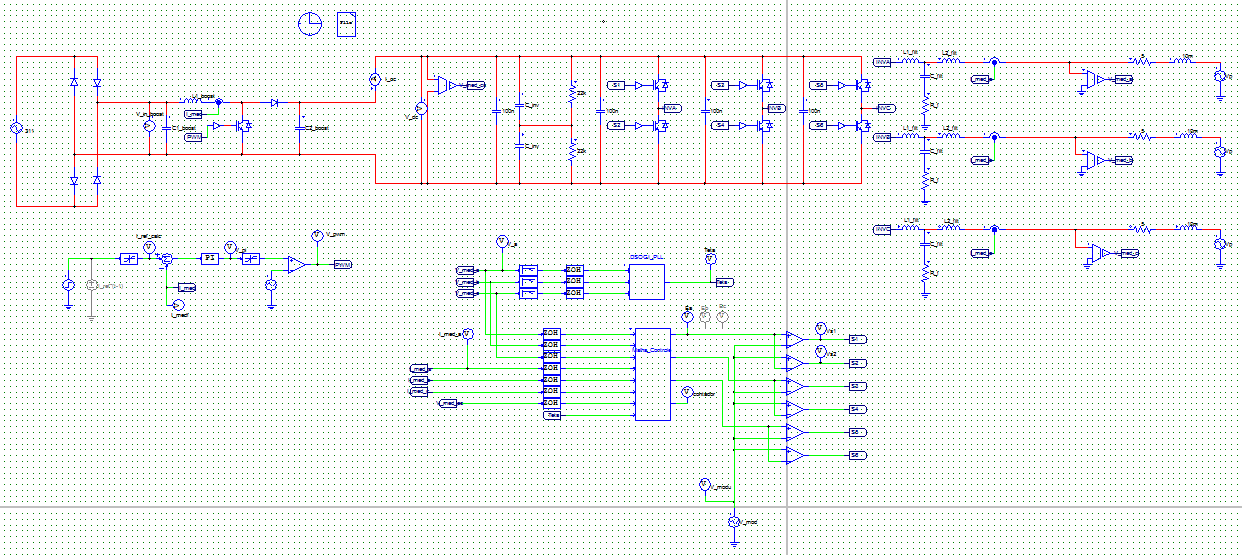
\includegraphics[width=\textwidth]{figuras/sim_figures/sistema_completo/montagem/sistema_completo.PNG}    \centering
    \caption{Circuito do inversor conectado com o conversor \textit{boost}, juntamente com os blocos de controle no software PSIM}
    \label{fig:sim-circuito-inversor-boost}
    \end{center}
\end{figure}

A tensão de referência definida para o barramento CC foi de 700 V. Desta forma, esperou-se que, apesar das pertubações a serem inseridas no sistema, este conseguisse estabilizar a tensão do barramento CC pŕoximo a tensão de referência após alguns segundos. 
Inicialmente o sistema foi inicializado sem nenhuma injeção de potência no barramento CC e permaneceu assim até os 4 segundos. Após, isso iniciou-se a injeção de potência.

O conversor \textit{boost} foi programado para injetar 10 A de corrente contínua constantes a partir de 4,0 segundos do tempo de simulação.

Pode-se verificar na Fig. \ref{fig:sim-tensao-barramento} a estabilização de tensão no barramento CC. 
Antes dos 4 segundos, o sistema passou por um transitório mas conseguiu manter a tensão no barramento próximo de 700 V. 
Após isto, houve a inserção de corrente pelo \textit{boost}, que provocou uma pertubação no barramento, de forma a elevar a tensão sobre o \textit{link} capacitivo do barramento.
De forma a estabilizar esta tensão, o sistema começou a fornecer potência à rede elétrica de modo a manter a tensão no barramento próximo ao valor de referência.

\begin{figure}[!hbt]
	\begin{center}
    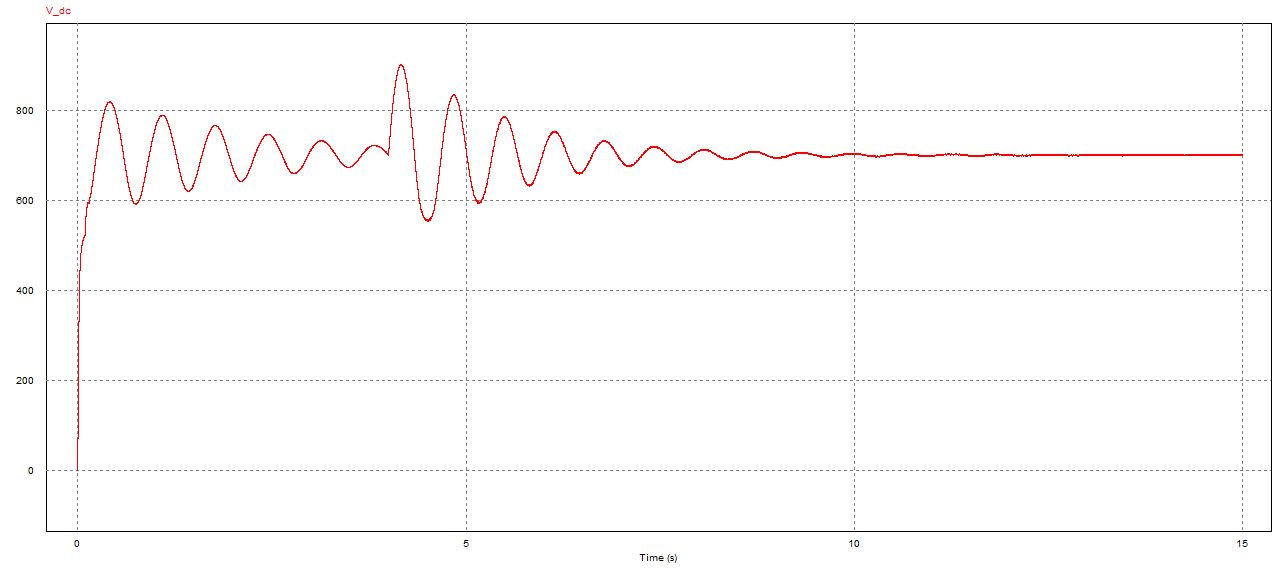
\includegraphics[width=\textwidth]{figuras/sim_figures/sistema_completo/tensao_barramento.PNG}
    \caption{Tensão no barramento CC. A tensão de referência foi definida como 700 V. Inicialmente este foi inicializado sem nenhuma injeção de potência no barramento, como pode-se verificar antes dos 4 segundos. A partir disso, acontece uma pertubação devido a injeção de potência, porém este consegue se estabilizar próximo a tensão de referência após alguns segundos}
    \label{fig:sim-tensao-barramento}
    \end{center}
\end{figure}

A Fig. \ref{fig:sim-tensao-saida-inversor} mostra as tensões sintetizadas na saída do inversor, após o filtro $L_2$.
Já a Fig. \ref{fig:sim-corrente-saida-inversor} mostra as correntes geradas após a inserção de potência pelo \textit{boost} no barramento CC.

\begin{figure}[!hbt]
	\centering
	\begin{subfigure}[b]{\textwidth}
		\centering
		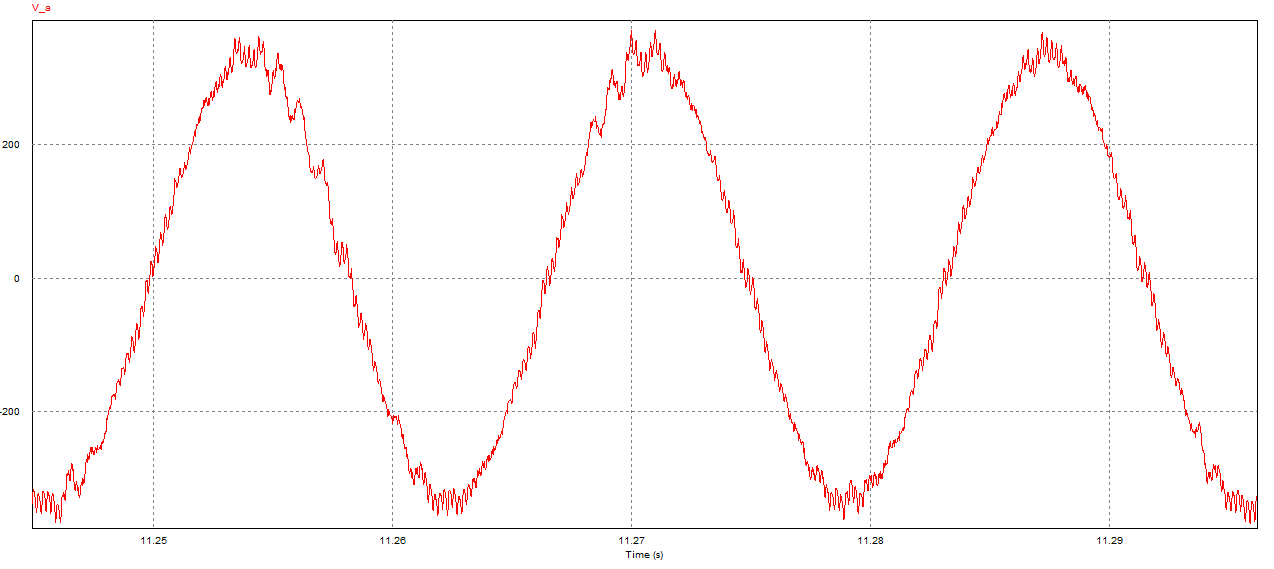
\includegraphics[width=\textwidth]{figuras/sim_figures/sistema_completo/tensao_saida_inversor_2.PNG}
		\caption{Tensão de saída sintetizada para a fase A}
    \end{subfigure}

    \begin{subfigure}[b]{\textwidth}
		\centering
		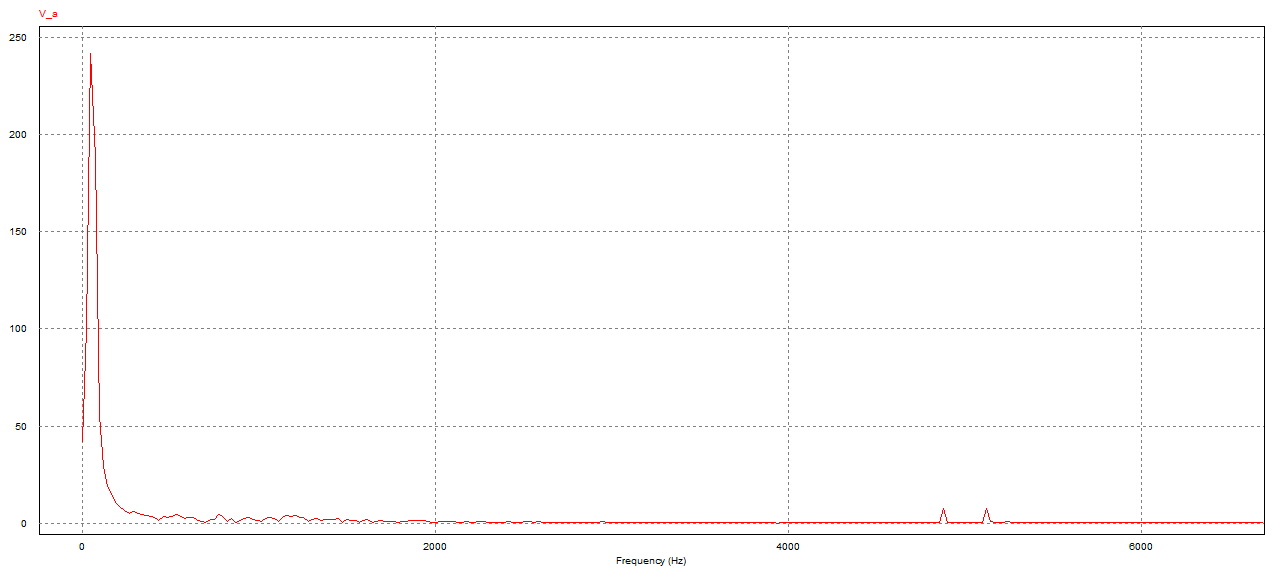
\includegraphics[width=\textwidth]{figuras/sim_figures/sistema_completo/tensao_saida_inversor_fft.PNG}
		\caption{Expectro em frequência da tensão sintetizada na fase A. Os harmônicos de alta frequência próximos a frequência de chaveamento de 5 kHz sofreram uma boa atenuação}
    \end{subfigure}

	\begin{subfigure}[b]{\textwidth}
		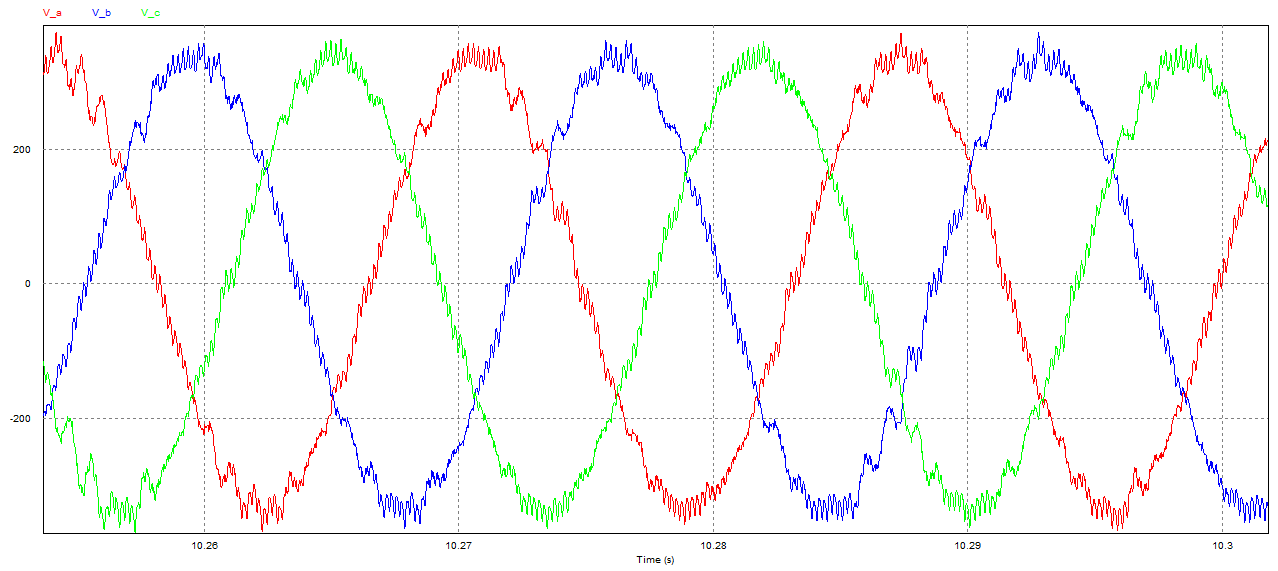
\includegraphics[width=\textwidth]{figuras/sim_figures/sistema_completo/tensao_saida_inversor_4.PNG}
		\caption{Tensões de saída sintetizadas para as fases A, B e C}
	\end{subfigure}
    \caption{Análise das tensões de saída sintetizadas após o filtro LCL}
    \label{fig:sim-tensao-saida-inversor}
\end{figure}

\begin{figure}[!hbt]
	\centering
	\begin{subfigure}[b]{\textwidth}
		\centering
		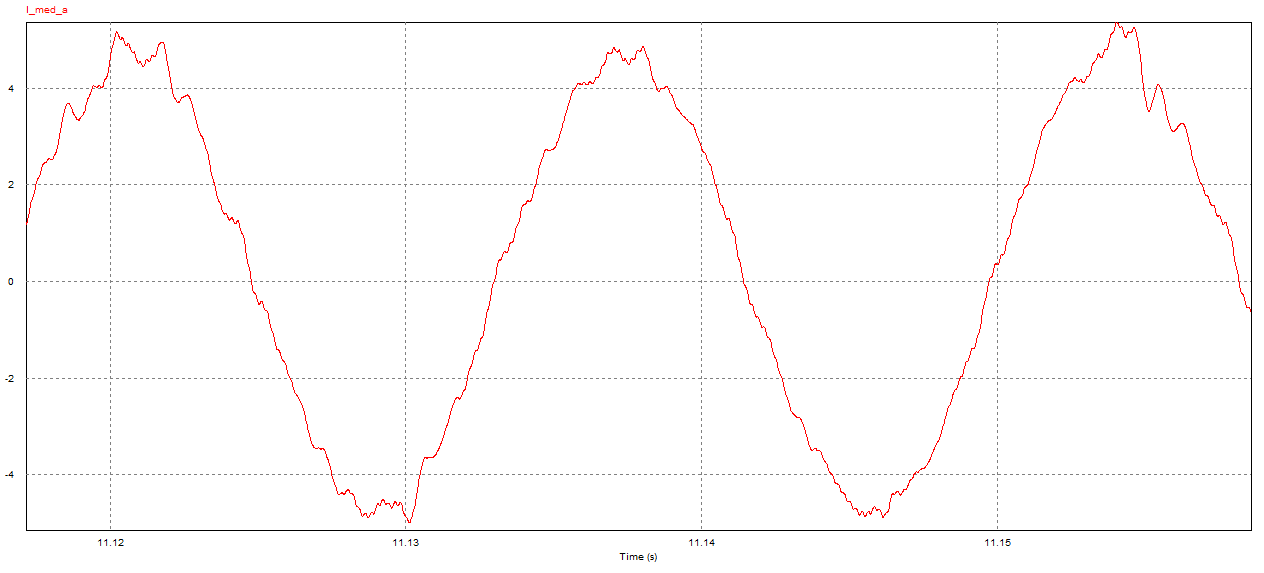
\includegraphics[width=\textwidth]{figuras/sim_figures/sistema_completo/corrente_saida_inversor_1.PNG}
		\caption{Corrente de saída na fase A}
    \end{subfigure}

    \begin{subfigure}[b]{\textwidth}
		\centering
		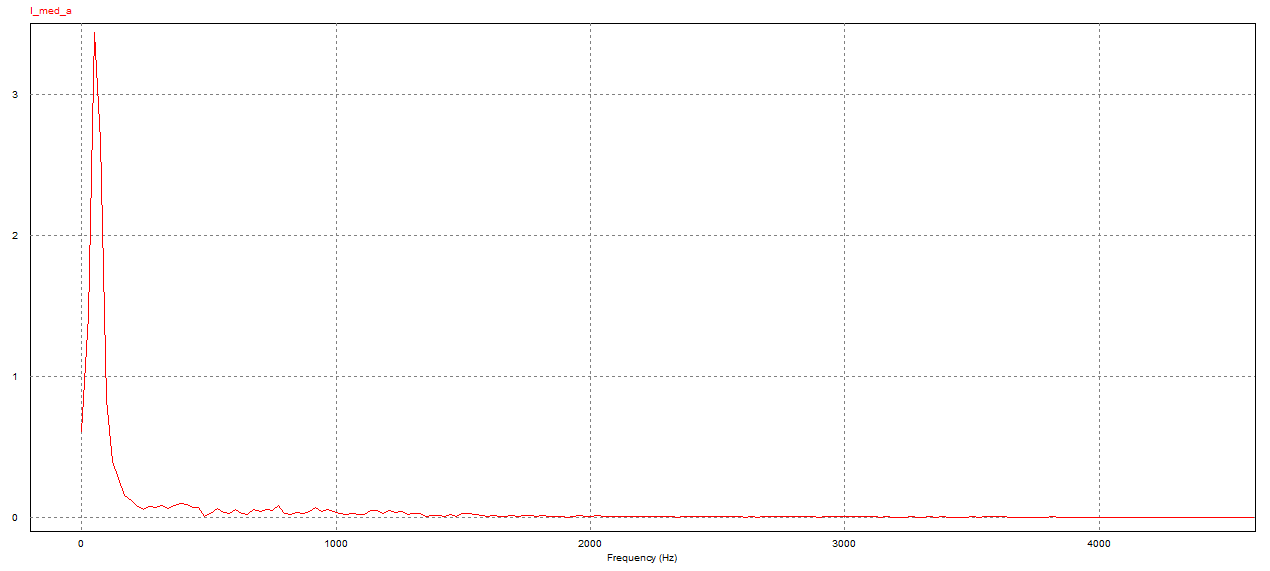
\includegraphics[width=\textwidth]{figuras/sim_figures/sistema_completo/corrente_saida_inversor_fft.PNG}
		\caption{Expectro em frequência da corrente na fase A. Os harmônicos de baixa frequência também sofreram uma boa atenuação}
    \end{subfigure}

	\begin{subfigure}[b]{\textwidth}
		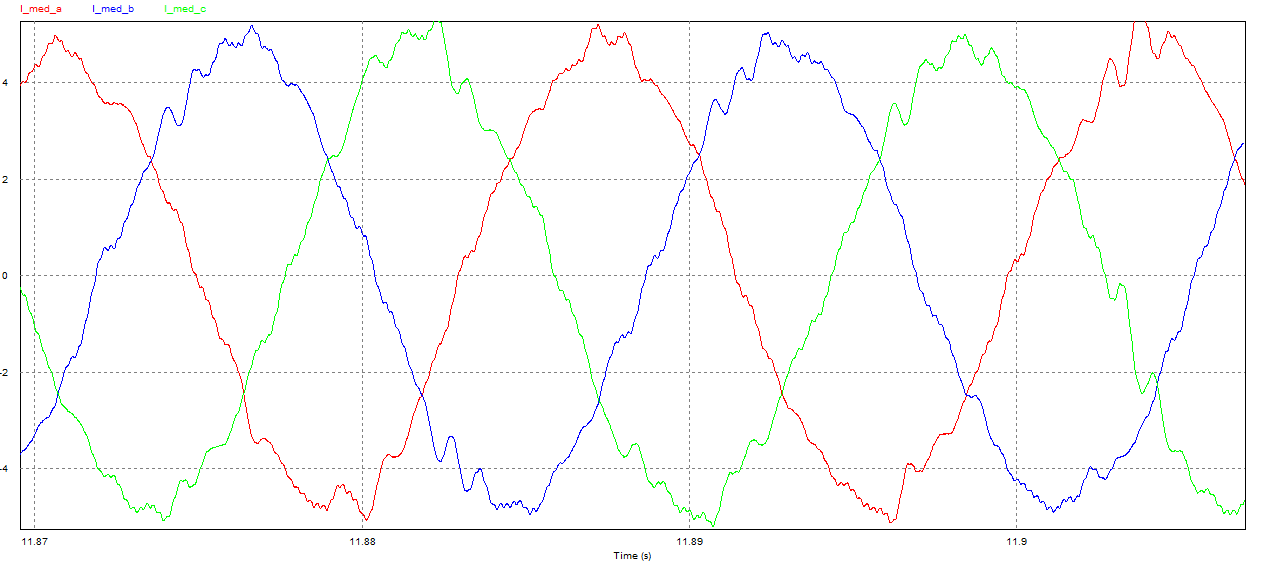
\includegraphics[width=\textwidth]{figuras/sim_figures/sistema_completo/corrente_saida_inversor_2.PNG}
		\caption{Correntes de saída para as fases A, B e C}
	\end{subfigure}
    \caption{Análise das corrente de saída após o filtro LCL. Estes resultados foram obtidos após a inserção de corrente pelo conversor \textit{boost} no barramento CC}
    \label{fig:sim-corrente-saida-inversor}
\end{figure}